% Options for packages loaded elsewhere
\PassOptionsToPackage{unicode}{hyperref}
\PassOptionsToPackage{hyphens}{url}
%
\documentclass[
]{article}
\usepackage{amsmath,amssymb}
\usepackage{lmodern}
\usepackage{iftex}
\ifPDFTeX
  \usepackage[T1]{fontenc}
  \usepackage[utf8]{inputenc}
  \usepackage{textcomp} % provide euro and other symbols
\else % if luatex or xetex
  \usepackage{unicode-math}
  \defaultfontfeatures{Scale=MatchLowercase}
  \defaultfontfeatures[\rmfamily]{Ligatures=TeX,Scale=1}
\fi
% Use upquote if available, for straight quotes in verbatim environments
\IfFileExists{upquote.sty}{\usepackage{upquote}}{}
\IfFileExists{microtype.sty}{% use microtype if available
  \usepackage[]{microtype}
  \UseMicrotypeSet[protrusion]{basicmath} % disable protrusion for tt fonts
}{}
\makeatletter
\@ifundefined{KOMAClassName}{% if non-KOMA class
  \IfFileExists{parskip.sty}{%
    \usepackage{parskip}
  }{% else
    \setlength{\parindent}{0pt}
    \setlength{\parskip}{6pt plus 2pt minus 1pt}}
}{% if KOMA class
  \KOMAoptions{parskip=half}}
\makeatother
\usepackage{xcolor}
\usepackage[margin=2.54cm]{geometry}
\usepackage{color}
\usepackage{fancyvrb}
\newcommand{\VerbBar}{|}
\newcommand{\VERB}{\Verb[commandchars=\\\{\}]}
\DefineVerbatimEnvironment{Highlighting}{Verbatim}{commandchars=\\\{\}}
% Add ',fontsize=\small' for more characters per line
\usepackage{framed}
\definecolor{shadecolor}{RGB}{248,248,248}
\newenvironment{Shaded}{\begin{snugshade}}{\end{snugshade}}
\newcommand{\AlertTok}[1]{\textcolor[rgb]{0.94,0.16,0.16}{#1}}
\newcommand{\AnnotationTok}[1]{\textcolor[rgb]{0.56,0.35,0.01}{\textbf{\textit{#1}}}}
\newcommand{\AttributeTok}[1]{\textcolor[rgb]{0.77,0.63,0.00}{#1}}
\newcommand{\BaseNTok}[1]{\textcolor[rgb]{0.00,0.00,0.81}{#1}}
\newcommand{\BuiltInTok}[1]{#1}
\newcommand{\CharTok}[1]{\textcolor[rgb]{0.31,0.60,0.02}{#1}}
\newcommand{\CommentTok}[1]{\textcolor[rgb]{0.56,0.35,0.01}{\textit{#1}}}
\newcommand{\CommentVarTok}[1]{\textcolor[rgb]{0.56,0.35,0.01}{\textbf{\textit{#1}}}}
\newcommand{\ConstantTok}[1]{\textcolor[rgb]{0.00,0.00,0.00}{#1}}
\newcommand{\ControlFlowTok}[1]{\textcolor[rgb]{0.13,0.29,0.53}{\textbf{#1}}}
\newcommand{\DataTypeTok}[1]{\textcolor[rgb]{0.13,0.29,0.53}{#1}}
\newcommand{\DecValTok}[1]{\textcolor[rgb]{0.00,0.00,0.81}{#1}}
\newcommand{\DocumentationTok}[1]{\textcolor[rgb]{0.56,0.35,0.01}{\textbf{\textit{#1}}}}
\newcommand{\ErrorTok}[1]{\textcolor[rgb]{0.64,0.00,0.00}{\textbf{#1}}}
\newcommand{\ExtensionTok}[1]{#1}
\newcommand{\FloatTok}[1]{\textcolor[rgb]{0.00,0.00,0.81}{#1}}
\newcommand{\FunctionTok}[1]{\textcolor[rgb]{0.00,0.00,0.00}{#1}}
\newcommand{\ImportTok}[1]{#1}
\newcommand{\InformationTok}[1]{\textcolor[rgb]{0.56,0.35,0.01}{\textbf{\textit{#1}}}}
\newcommand{\KeywordTok}[1]{\textcolor[rgb]{0.13,0.29,0.53}{\textbf{#1}}}
\newcommand{\NormalTok}[1]{#1}
\newcommand{\OperatorTok}[1]{\textcolor[rgb]{0.81,0.36,0.00}{\textbf{#1}}}
\newcommand{\OtherTok}[1]{\textcolor[rgb]{0.56,0.35,0.01}{#1}}
\newcommand{\PreprocessorTok}[1]{\textcolor[rgb]{0.56,0.35,0.01}{\textit{#1}}}
\newcommand{\RegionMarkerTok}[1]{#1}
\newcommand{\SpecialCharTok}[1]{\textcolor[rgb]{0.00,0.00,0.00}{#1}}
\newcommand{\SpecialStringTok}[1]{\textcolor[rgb]{0.31,0.60,0.02}{#1}}
\newcommand{\StringTok}[1]{\textcolor[rgb]{0.31,0.60,0.02}{#1}}
\newcommand{\VariableTok}[1]{\textcolor[rgb]{0.00,0.00,0.00}{#1}}
\newcommand{\VerbatimStringTok}[1]{\textcolor[rgb]{0.31,0.60,0.02}{#1}}
\newcommand{\WarningTok}[1]{\textcolor[rgb]{0.56,0.35,0.01}{\textbf{\textit{#1}}}}
\usepackage{graphicx}
\makeatletter
\def\maxwidth{\ifdim\Gin@nat@width>\linewidth\linewidth\else\Gin@nat@width\fi}
\def\maxheight{\ifdim\Gin@nat@height>\textheight\textheight\else\Gin@nat@height\fi}
\makeatother
% Scale images if necessary, so that they will not overflow the page
% margins by default, and it is still possible to overwrite the defaults
% using explicit options in \includegraphics[width, height, ...]{}
\setkeys{Gin}{width=\maxwidth,height=\maxheight,keepaspectratio}
% Set default figure placement to htbp
\makeatletter
\def\fps@figure{htbp}
\makeatother
\setlength{\emergencystretch}{3em} % prevent overfull lines
\providecommand{\tightlist}{%
  \setlength{\itemsep}{0pt}\setlength{\parskip}{0pt}}
\setcounter{secnumdepth}{-\maxdimen} % remove section numbering
\usepackage{booktabs}
\usepackage{longtable}
\usepackage{array}
\usepackage{multirow}
\usepackage{wrapfig}
\usepackage{float}
\usepackage{colortbl}
\usepackage{pdflscape}
\usepackage{tabu}
\usepackage{threeparttable}
\usepackage{threeparttablex}
\usepackage[normalem]{ulem}
\usepackage{makecell}
\usepackage{xcolor}
\ifLuaTeX
  \usepackage{selnolig}  % disable illegal ligatures
\fi
\IfFileExists{bookmark.sty}{\usepackage{bookmark}}{\usepackage{hyperref}}
\IfFileExists{xurl.sty}{\usepackage{xurl}}{} % add URL line breaks if available
\urlstyle{same} % disable monospaced font for URLs
\hypersetup{
  pdftitle={ENV 790.30 - Time Series Analysis for Energy Data \textbar{} Spring 2023},
  pdfauthor={John Rooney},
  hidelinks,
  pdfcreator={LaTeX via pandoc}}

\title{ENV 790.30 - Time Series Analysis for Energy Data \textbar{}
Spring 2023}
\usepackage{etoolbox}
\makeatletter
\providecommand{\subtitle}[1]{% add subtitle to \maketitle
  \apptocmd{\@title}{\par {\large #1 \par}}{}{}
}
\makeatother
\subtitle{Assignment 8 - Due date 03/27/23}
\author{John Rooney}
\date{}

\begin{document}
\maketitle

\hypertarget{directions}{%
\subsection{Directions}\label{directions}}

You should open the .rmd file corresponding to this assignment on
RStudio. The file is available on our class repository on Github. And to
do so you will need to fork our repository and link it to your RStudio.

Once you have the project open the first thing you will do is change
``Student Name'' on line 3 with your name. Then you will start working
through the assignment by \textbf{creating code and output} that answer
each question. Be sure to use this assignment document. Your report
should contain the answer to each question and any plots/tables you
obtained (when applicable).

When you have completed the assignment, \textbf{Knit} the text and code
into a single PDF file. Rename the pdf file such that it includes your
first and last name (e.g., ``LuanaLima\_TSA\_A08\_Sp22.Rmd''). Submit
this pdf using Sakai.

\hypertarget{set-up}{%
\subsection{Set up}\label{set-up}}

Some packages needed for this assignment:
\texttt{forecast},\texttt{tseries},\texttt{smooth}. Do not forget to
load them before running your script, since they are NOT default
packages.

\begin{Shaded}
\begin{Highlighting}[]
\CommentTok{\#Load/install required package here}
\FunctionTok{library}\NormalTok{(forecast)}
\end{Highlighting}
\end{Shaded}

\begin{verbatim}
## Registered S3 method overwritten by 'quantmod':
##   method            from
##   as.zoo.data.frame zoo
\end{verbatim}

\begin{Shaded}
\begin{Highlighting}[]
\FunctionTok{library}\NormalTok{(tseries)}
\FunctionTok{library}\NormalTok{(smooth)}
\end{Highlighting}
\end{Shaded}

\begin{verbatim}
## Loading required package: greybox
\end{verbatim}

\begin{verbatim}
## Package "greybox", v1.0.7 loaded.
\end{verbatim}

\begin{verbatim}
## This is package "smooth", v3.2.0
\end{verbatim}

\begin{Shaded}
\begin{Highlighting}[]
\FunctionTok{library}\NormalTok{(here)}
\end{Highlighting}
\end{Shaded}

\begin{verbatim}
## here() starts at /Users/jrooney/Library/Mobile Documents/com~apple~CloudDocs/TSA_Sp23_new
\end{verbatim}

\begin{Shaded}
\begin{Highlighting}[]
\FunctionTok{library}\NormalTok{(lubridate)}
\end{Highlighting}
\end{Shaded}

\begin{verbatim}
## 
## Attaching package: 'lubridate'
\end{verbatim}

\begin{verbatim}
## The following object is masked from 'package:greybox':
## 
##     hm
\end{verbatim}

\begin{verbatim}
## The following objects are masked from 'package:base':
## 
##     date, intersect, setdiff, union
\end{verbatim}

\begin{Shaded}
\begin{Highlighting}[]
\FunctionTok{library}\NormalTok{(tidyverse)}
\end{Highlighting}
\end{Shaded}

\begin{verbatim}
## -- Attaching packages --------------------------------------- tidyverse 1.3.2 --
\end{verbatim}

\begin{verbatim}
## v ggplot2 3.4.0     v purrr   1.0.1
## v tibble  3.1.8     v dplyr   1.1.0
## v tidyr   1.3.0     v stringr 1.5.0
## v readr   2.1.3     v forcats 1.0.0
## -- Conflicts ------------------------------------------ tidyverse_conflicts() --
## x lubridate::as.difftime() masks base::as.difftime()
## x lubridate::date()        masks base::date()
## x dplyr::filter()          masks stats::filter()
## x lubridate::hm()          masks greybox::hm()
## x lubridate::intersect()   masks base::intersect()
## x dplyr::lag()             masks stats::lag()
## x lubridate::setdiff()     masks base::setdiff()
## x tidyr::spread()          masks greybox::spread()
## x lubridate::union()       masks base::union()
\end{verbatim}

\begin{Shaded}
\begin{Highlighting}[]
\FunctionTok{library}\NormalTok{(kableExtra)}
\end{Highlighting}
\end{Shaded}

\begin{verbatim}
## 
## Attaching package: 'kableExtra'
## 
## The following object is masked from 'package:dplyr':
## 
##     group_rows
\end{verbatim}

\hypertarget{importing-and-processing-the-data-set}{%
\subsection{Importing and processing the data
set}\label{importing-and-processing-the-data-set}}

Consider the data from the file ``inflowtimeseries.txt''. The data
corresponds to the monthly inflow in \(m^{3}/s\) for some hydro power
plants in Brazil. You will only use the last column of the data set
which represents one hydro plant in the Amazon river basin. The data
span the period from January 1931 to August 2011 and is provided by the
Brazilian ISO.

For all parts of the assignment prepare the data set such that the model
consider only the data from January 2000 up to December 2009. Leave the
year 2010 of data (January 2010 to December 2010) for the out-of-sample
analysis. Do \textbf{NOT} use data fro 2010 and 2011 for model fitting.
You will only use it to compute forecast accuracy of your model.

\hypertarget{part-i-preparing-the-data-sets}{%
\subsection{Part I: Preparing the data
sets}\label{part-i-preparing-the-data-sets}}

\hypertarget{q1}{%
\subsubsection{Q1}\label{q1}}

Read the file into a data frame. Prepare your time series data vector
such that observations start in January 2000 and end in December 2009.
Make you sure you specify the \textbf{start=} and \textbf{frequency=}
arguments. Plot the time series over time, ACF and PACF.

\begin{Shaded}
\begin{Highlighting}[]
\CommentTok{\#read file into data frame}
\NormalTok{data }\OtherTok{=} \StringTok{"Data/"}
\NormalTok{raw\_inflow\_data }\OtherTok{\textless{}{-}} \FunctionTok{read.table}\NormalTok{(}
  \FunctionTok{here}\NormalTok{(data, }\StringTok{"inflowtimeseries.txt"}\NormalTok{), }\AttributeTok{header=}\NormalTok{F, }\AttributeTok{sep =} \StringTok{""}\NormalTok{) }

\CommentTok{\#add column names}
\FunctionTok{colnames}\NormalTok{(raw\_inflow\_data)}\OtherTok{=}\FunctionTok{c}\NormalTok{(}\StringTok{"Month"}\NormalTok{,}\StringTok{"Year"}\NormalTok{, }\StringTok{"HP1"}\NormalTok{, }\StringTok{"HP2"}\NormalTok{,}\StringTok{"HP3"}\NormalTok{,}\StringTok{"HP4"}\NormalTok{, }\StringTok{"HP5"}\NormalTok{,}
                            \StringTok{"HP6"}\NormalTok{,}\StringTok{"HP7"}\NormalTok{, }\StringTok{"HP8"}\NormalTok{,}\StringTok{"HP9"}\NormalTok{,}\StringTok{"HP10"}\NormalTok{, }\StringTok{"HP11"}\NormalTok{,}\StringTok{"HP12"}\NormalTok{, }
                            \StringTok{"HP13"}\NormalTok{, }\StringTok{"HP14"}\NormalTok{,}\StringTok{"HP15"}\NormalTok{)}


\CommentTok{\#wrangle data sets}
\NormalTok{inflow\_data\_test }\OtherTok{\textless{}{-}}
\NormalTok{  raw\_inflow\_data }\SpecialCharTok{\%\textgreater{}\%}
\NormalTok{  dplyr}\SpecialCharTok{::}\FunctionTok{filter}\NormalTok{(Year }\SpecialCharTok{\textgreater{}=} \DecValTok{2000} \SpecialCharTok{\&}\NormalTok{ Year }\SpecialCharTok{\textless{}=} \DecValTok{2009}\NormalTok{) }\SpecialCharTok{\%\textgreater{}\%}
\NormalTok{  dplyr}\SpecialCharTok{::}\FunctionTok{select}\NormalTok{(Month, Year, HP15)}

\NormalTok{inflow\_data\_full }\OtherTok{\textless{}{-}} 
\NormalTok{  raw\_inflow\_data }\SpecialCharTok{\%\textgreater{}\%}
  \FunctionTok{filter}\NormalTok{(Year }\SpecialCharTok{\textgreater{}=} \DecValTok{2000} \SpecialCharTok{\&}\NormalTok{ Year }\SpecialCharTok{\textless{}=} \DecValTok{2010}\NormalTok{) }\SpecialCharTok{\%\textgreater{}\%}
  \FunctionTok{select}\NormalTok{(Month, Year, HP15)}



\CommentTok{\#make a time series for HP15 from January 2000 to December 2009}
\NormalTok{ts\_inflow\_test }\OtherTok{\textless{}{-}} \FunctionTok{ts}\NormalTok{(inflow\_data\_test[,}\DecValTok{3}\NormalTok{], }\AttributeTok{start=}\FunctionTok{c}\NormalTok{(}\DecValTok{2000}\NormalTok{,}\DecValTok{1}\NormalTok{), }\AttributeTok{frequency=}\DecValTok{12}\NormalTok{) }

\NormalTok{ts\_inflow\_full }\OtherTok{\textless{}{-}} \FunctionTok{ts}\NormalTok{(inflow\_data\_full[,}\DecValTok{3}\NormalTok{], }\AttributeTok{start=}\FunctionTok{c}\NormalTok{(}\DecValTok{2000}\NormalTok{,}\DecValTok{1}\NormalTok{), }\AttributeTok{frequency=}\DecValTok{12}\NormalTok{)}

\CommentTok{\#plot the time series}
\FunctionTok{plot}\NormalTok{(ts\_inflow\_test)}
\end{Highlighting}
\end{Shaded}

\includegraphics{JohnRooney_TSA_A08_Sp23_files/figure-latex/unnamed-chunk-2-1.pdf}

\begin{Shaded}
\begin{Highlighting}[]
\CommentTok{\#Acf and Pacf for HP15}
\FunctionTok{Acf}\NormalTok{(ts\_inflow\_test,}\AttributeTok{lag.max=}\DecValTok{40}\NormalTok{,}\AttributeTok{main=}\FunctionTok{paste}\NormalTok{(}\StringTok{"Inflows HP15"}\NormalTok{,}\AttributeTok{sep=}\StringTok{""}\NormalTok{)) }
\end{Highlighting}
\end{Shaded}

\includegraphics{JohnRooney_TSA_A08_Sp23_files/figure-latex/unnamed-chunk-2-2.pdf}

\begin{Shaded}
\begin{Highlighting}[]
\FunctionTok{Pacf}\NormalTok{(ts\_inflow\_test,}\AttributeTok{lag.max=}\DecValTok{40}\NormalTok{,}\AttributeTok{main=}\FunctionTok{paste}\NormalTok{(}\StringTok{"Inflows HP15"}\NormalTok{,}\AttributeTok{sep=}\StringTok{""}\NormalTok{))}
\end{Highlighting}
\end{Shaded}

\includegraphics{JohnRooney_TSA_A08_Sp23_files/figure-latex/unnamed-chunk-2-3.pdf}

\hypertarget{q2}{%
\subsubsection{Q2}\label{q2}}

Using the \(decompose()\) or \(stl()\) and the \(seasadj()\) functions
create a series without the seasonal component, i.e., a deseasonalized
inflow series. Plot the deseasonalized series and original series
together using ggplot, make sure your plot includes a legend. Plot ACF
and PACF for the deaseasonalized series. Compare with the plots obtained
in Q1.

\begin{Shaded}
\begin{Highlighting}[]
\CommentTok{\#decompose the time series}
\NormalTok{decomp\_inflow\_test }\OtherTok{\textless{}{-}} \FunctionTok{decompose}\NormalTok{(ts\_inflow\_test, }\StringTok{"additive"}\NormalTok{)}

\NormalTok{decomp\_inflow\_full }\OtherTok{\textless{}{-}} \FunctionTok{decompose}\NormalTok{(ts\_inflow\_full, }\StringTok{"additive"}\NormalTok{)}

\NormalTok{deseason\_inflow\_test }\OtherTok{\textless{}{-}} \FunctionTok{seasadj}\NormalTok{(decomp\_inflow\_test)}

\NormalTok{deseason\_inflow\_full }\OtherTok{\textless{}{-}} \FunctionTok{seasadj}\NormalTok{(decomp\_inflow\_full)}

\CommentTok{\#plot deseasonalized and original series}
\FunctionTok{autoplot}\NormalTok{(ts\_inflow\_full) }\SpecialCharTok{+}
  \FunctionTok{autolayer}\NormalTok{(deseason\_inflow\_full, }\AttributeTok{series=}\StringTok{"Deseason"}\NormalTok{)}
\end{Highlighting}
\end{Shaded}

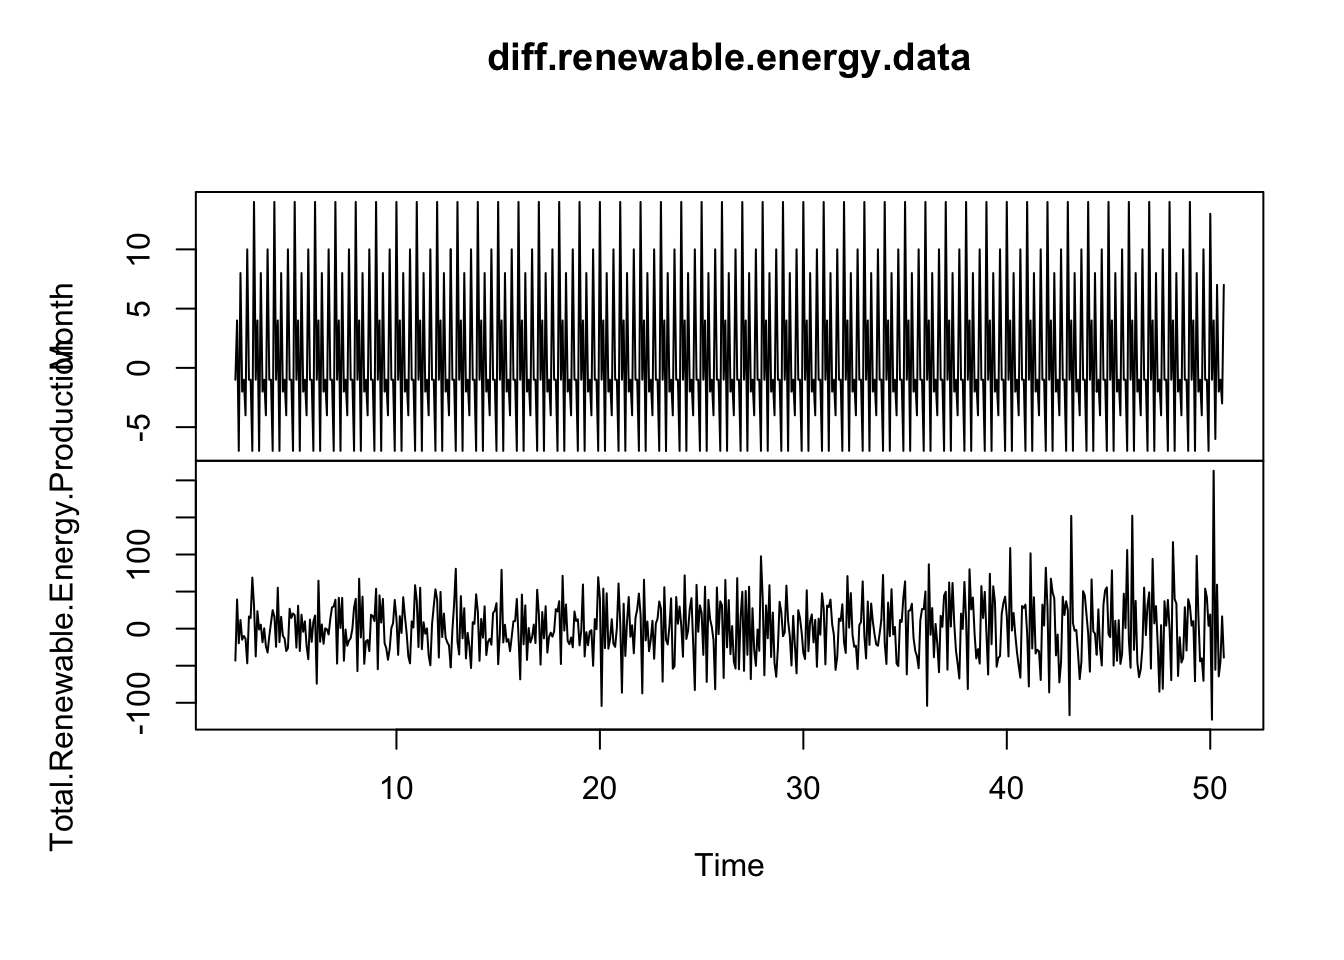
\includegraphics{JohnRooney_TSA_A08_Sp23_files/figure-latex/unnamed-chunk-3-1.pdf}

\begin{Shaded}
\begin{Highlighting}[]
\CommentTok{\#deseasonal\_and\_original\_plot}

\CommentTok{\#ACF and PACF}
\FunctionTok{Acf}\NormalTok{(deseason\_inflow\_full,}\AttributeTok{lag.max=}\DecValTok{40}\NormalTok{,}\AttributeTok{main=}\FunctionTok{paste}\NormalTok{(}\StringTok{"Deseasoned Inflows HP15"}\NormalTok{,}\AttributeTok{sep=}\StringTok{""}\NormalTok{)) }
\end{Highlighting}
\end{Shaded}

\includegraphics{JohnRooney_TSA_A08_Sp23_files/figure-latex/unnamed-chunk-3-2.pdf}

\begin{Shaded}
\begin{Highlighting}[]
\FunctionTok{Pacf}\NormalTok{(deseason\_inflow\_full,}\AttributeTok{lag.max=}\DecValTok{40}\NormalTok{,}\AttributeTok{main=}\FunctionTok{paste}\NormalTok{(}\StringTok{"Inflows HP15"}\NormalTok{,}\AttributeTok{sep=}\StringTok{""}\NormalTok{))}
\end{Highlighting}
\end{Shaded}

\includegraphics{JohnRooney_TSA_A08_Sp23_files/figure-latex/unnamed-chunk-3-3.pdf}

\hypertarget{part-ii-forecasting-with-arima-models-and-its-variations}{%
\subsection{Part II: Forecasting with ARIMA models and its
variations}\label{part-ii-forecasting-with-arima-models-and-its-variations}}

\hypertarget{q3}{%
\subsubsection{Q3}\label{q3}}

Fit a non-seasonal ARIMA\((p,d,q)\) model using the auto.arima()
function to the non-seasonal data. Forecast 12 months ahead of time
using the \(forecast()\) function. Plot your forecasting results and
further include on the plot the last year of non-seasonal data to
compare with forecasted values (similar to the plot on the lesson file
for M9).

\begin{Shaded}
\begin{Highlighting}[]
\CommentTok{\#fit non{-}seasonal ARIMA model and forecast}
\NormalTok{ARIMA\_autofit }\OtherTok{\textless{}{-}} \FunctionTok{auto.arima}\NormalTok{(deseason\_inflow\_test, }\AttributeTok{max.D =} \DecValTok{0}\NormalTok{, }\AttributeTok{max.P =} \DecValTok{0}\NormalTok{, }\AttributeTok{max.Q =} \DecValTok{0}\NormalTok{)}
\FunctionTok{print}\NormalTok{(ARIMA\_autofit)}
\end{Highlighting}
\end{Shaded}

\begin{verbatim}
## Series: deseason_inflow_test 
## ARIMA(0,1,0) 
## 
## sigma^2 = 5031380:  log likelihood = -1087.01
## AIC=2176.02   AICc=2176.05   BIC=2178.8
\end{verbatim}

\begin{Shaded}
\begin{Highlighting}[]
\NormalTok{ARIMA\_forecast }\OtherTok{\textless{}{-}} \FunctionTok{forecast}\NormalTok{(}\AttributeTok{object =}\NormalTok{ ARIMA\_autofit, }\AttributeTok{h =} \DecValTok{12}\NormalTok{)}
\FunctionTok{plot}\NormalTok{(ARIMA\_forecast)}
\end{Highlighting}
\end{Shaded}

\includegraphics{JohnRooney_TSA_A08_Sp23_files/figure-latex/unnamed-chunk-4-1.pdf}

\begin{Shaded}
\begin{Highlighting}[]
\CommentTok{\#plot forecast and last year of non{-}seasonal data}

\FunctionTok{autoplot}\NormalTok{(deseason\_inflow\_full) }\SpecialCharTok{+}
  \FunctionTok{autolayer}\NormalTok{(ARIMA\_forecast, }\AttributeTok{series=}\StringTok{"ARIMA Forecast without Seasonality"}\NormalTok{)}
\end{Highlighting}
\end{Shaded}

\includegraphics{JohnRooney_TSA_A08_Sp23_files/figure-latex/unnamed-chunk-4-2.pdf}

\hypertarget{q4}{%
\subsubsection{Q4}\label{q4}}

Put the seasonality back on your forecasted values and compare with the
original seasonal data values. \(Hint:\) One way to do it is by summing
the last year of the seasonal component from your decompose object to
the forecasted series.

\begin{Shaded}
\begin{Highlighting}[]
\NormalTok{seasonal }\OtherTok{\textless{}{-}}\NormalTok{ ts\_inflow\_full }\SpecialCharTok{{-}}\NormalTok{ deseason\_inflow\_full}

\NormalTok{new\_ARIMA\_forecast }\OtherTok{\textless{}{-}}\NormalTok{ ARIMA\_forecast}\SpecialCharTok{$}\NormalTok{mean }\SpecialCharTok{+}\NormalTok{ seasonal[}\DecValTok{1}\SpecialCharTok{:}\DecValTok{12}\NormalTok{]}

\FunctionTok{autoplot}\NormalTok{(ts\_inflow\_full) }\SpecialCharTok{+}
  \FunctionTok{autolayer}\NormalTok{(new\_ARIMA\_forecast, }\AttributeTok{series =} \StringTok{"ARIMA Forecast with Seasonality"}\NormalTok{) }
\end{Highlighting}
\end{Shaded}

\includegraphics{JohnRooney_TSA_A08_Sp23_files/figure-latex/unnamed-chunk-5-1.pdf}

\hypertarget{q5}{%
\subsubsection{Q5}\label{q5}}

Repeat Q3 for the original data, but now fit a seasonal
ARIMA\((p,d,q)x(P,D,Q)_ {12}\) also using the auto.arima().

\begin{Shaded}
\begin{Highlighting}[]
\NormalTok{SARIMA\_autofit }\OtherTok{\textless{}{-}} \FunctionTok{auto.arima}\NormalTok{(ts\_inflow\_test)}
\FunctionTok{print}\NormalTok{(SARIMA\_autofit)}
\end{Highlighting}
\end{Shaded}

\begin{verbatim}
## Series: ts_inflow_test 
## ARIMA(1,0,0)(0,1,1)[12] with drift 
## 
## Coefficients:
##          ar1     sma1    drift
##       0.7739  -0.8724  54.7963
## s.e.  0.0614   0.1767  25.8402
## 
## sigma^2 = 5566545:  log likelihood = -999.07
## AIC=2006.14   AICc=2006.52   BIC=2016.86
\end{verbatim}

\begin{Shaded}
\begin{Highlighting}[]
\NormalTok{SARIMA\_forecast }\OtherTok{\textless{}{-}} \FunctionTok{forecast}\NormalTok{(}\AttributeTok{object =}\NormalTok{ SARIMA\_autofit, }\AttributeTok{h =} \DecValTok{12}\NormalTok{)}
\FunctionTok{plot}\NormalTok{(SARIMA\_forecast)}
\end{Highlighting}
\end{Shaded}

\includegraphics{JohnRooney_TSA_A08_Sp23_files/figure-latex/unnamed-chunk-6-1.pdf}

\hypertarget{q6}{%
\subsubsection{Q6}\label{q6}}

Compare the plots from Q4 and Q5 using the autoplot() function.

\begin{Shaded}
\begin{Highlighting}[]
\FunctionTok{autoplot}\NormalTok{(ts\_inflow\_full)}\SpecialCharTok{+}
  \FunctionTok{autolayer}\NormalTok{(new\_ARIMA\_forecast, }\AttributeTok{series =} \StringTok{"ARIMA Forecast with Seasonality"}\NormalTok{) }\SpecialCharTok{+}
  \FunctionTok{autolayer}\NormalTok{(SARIMA\_forecast, }\AttributeTok{series =} \StringTok{"SARMIA Forecast"}\NormalTok{, }\AttributeTok{alpha=}\FloatTok{0.5}\NormalTok{)}
\end{Highlighting}
\end{Shaded}

\includegraphics{JohnRooney_TSA_A08_Sp23_files/figure-latex/unnamed-chunk-7-1.pdf}

\hypertarget{part-iii-forecasting-with-other-models}{%
\subsection{Part III: Forecasting with Other
Models}\label{part-iii-forecasting-with-other-models}}

\hypertarget{q7}{%
\subsubsection{Q7}\label{q7}}

Fit an exponential smooth model to the original time series using the
function \(ses()\) from package \texttt{forecast}. Note that this
function automatically do the forecast. Do not forget to set the
arguments: silent=FALSE and holdout=FALSE, so that the plot is produced
and the forecast is for the year of 2010.

\begin{Shaded}
\begin{Highlighting}[]
\NormalTok{SES\_seas\_fit }\OtherTok{\textless{}{-}} \FunctionTok{ses}\NormalTok{(}\AttributeTok{y =}\NormalTok{ ts\_inflow\_test, }\AttributeTok{h =} \DecValTok{12}\NormalTok{, }\AttributeTok{holdout =} \ConstantTok{FALSE}\NormalTok{, }\AttributeTok{silent =} \ConstantTok{FALSE}\NormalTok{)}
\FunctionTok{summary}\NormalTok{(SES\_seas\_fit)}
\end{Highlighting}
\end{Shaded}

\begin{verbatim}
## 
## Forecast method: Simple exponential smoothing
## 
## Model Information:
## Simple exponential smoothing 
## 
## Call:
##  ses(y = ts_inflow_test, h = 12, holdout = FALSE, silent = FALSE) 
## 
##   Smoothing parameters:
##     alpha = 0.9999 
## 
##   Initial states:
##     l = 21885.2463 
## 
##   sigma:  6813.76
## 
##      AIC     AICc      BIC 
## 2696.890 2697.097 2705.252 
## 
## Error measures:
##                    ME    RMSE      MAE      MPE     MAPE     MASE      ACF1
## Training set 14.14103 6756.74 5787.733 -7.09394 34.05251 1.758853 0.7154525
## 
## Forecasts:
##          Point Forecast      Lo 80    Hi 80      Lo 95    Hi 95
## Jan 2010          23582 14849.8153 32314.19  10227.276 36936.72
## Feb 2010          23582 11233.4433 35930.56   4696.512 42467.49
## Mar 2010          23582  8458.4205 38705.58    452.481 46711.52
## Apr 2010          23582  6118.9402 41045.06  -3125.445 50289.45
## May 2010          23582  4057.8032 43106.20  -6277.682 53441.68
## Jun 2010          23582  2194.3852 44969.62  -9127.534 56291.53
## Jul 2010          23582   480.7907 46683.21 -11748.251 58912.25
## Aug 2010          23582 -1114.1874 48278.19 -14187.559 61351.56
## Sep 2010          23582 -2612.2260 49776.23 -16478.612 63642.61
## Oct 2010          23582 -4029.1079 51193.11 -18645.546 65809.55
## Nov 2010          23582 -5376.7480 52540.75 -20706.583 67870.58
## Dec 2010          23582 -6664.4029 53828.40 -22675.882 69839.88
\end{verbatim}

\begin{Shaded}
\begin{Highlighting}[]
\FunctionTok{plot}\NormalTok{(SES\_seas\_fit)}
\end{Highlighting}
\end{Shaded}

\includegraphics{JohnRooney_TSA_A08_Sp23_files/figure-latex/unnamed-chunk-8-1.pdf}

\hypertarget{part-iv-checking-forecast-accuracy}{%
\subsection{Part IV: Checking Forecast
Accuracy}\label{part-iv-checking-forecast-accuracy}}

\hypertarget{q8}{%
\subsubsection{Q8}\label{q8}}

Make one plot with the complete original seasonal historical data (Jan
2000 to Dec 2010). Now add the forecasts from each of the developed
models in parts Q4, Q5, Q7 and Q8. You can do it using the autoplot()
combined with autolayer(). If everything is correct in terms of time
line, the forecasted lines should appear only in the final year. If you
decide to use ggplot() you will need to create a data frame with all the
series will need to plot. Remember to use a different color for each
model and add a legend in the end to tell which forecast lines
corresponds to each model.

\begin{Shaded}
\begin{Highlighting}[]
\FunctionTok{autoplot}\NormalTok{(ts\_inflow\_full) }\SpecialCharTok{+}
  \FunctionTok{autolayer}\NormalTok{(new\_ARIMA\_forecast, }\AttributeTok{series =} \StringTok{"ARIMA Forecast with Seasonality"}\NormalTok{) }\SpecialCharTok{+}
  \FunctionTok{autolayer}\NormalTok{(SARIMA\_forecast, }\AttributeTok{series =} \StringTok{"SARMIA Forecast"}\NormalTok{, }\AttributeTok{alpha =}\FloatTok{0.3}\NormalTok{) }\SpecialCharTok{+}
  \FunctionTok{autolayer}\NormalTok{(SES\_seas\_fit, }\AttributeTok{series =} \StringTok{"Simple Exponential Smoothing Forecast"}\NormalTok{, }\AttributeTok{alpha=}\FloatTok{0.3}\NormalTok{)}
\end{Highlighting}
\end{Shaded}

\includegraphics{JohnRooney_TSA_A08_Sp23_files/figure-latex/unnamed-chunk-9-1.pdf}

\hypertarget{q9}{%
\subsubsection{Q9}\label{q9}}

From the plot in Q8 which model or model(s) are leading to the better
forecasts? Explain your answer. Hint: Think about which models are doing
a better job forecasting the high and low inflow months for example.

\begin{quote}
Answer: The Sarima model led to the best forecast. While it forecast
values higher then the peak and lower then the valley of the actual
data, it was closer then the ARIMA with seasonality and far better then
the SES model.
\end{quote}

\hypertarget{q10}{%
\subsubsection{Q10}\label{q10}}

Now compute the following forecast metrics we learned in class: RMSE and
MAPE, for all the models you plotted in part Q9. You can do this by hand
since you have forecasted and observed values for the year of 2010. Or
you can use R function \(accuracy()\) from package ``forecast'' to do
it. Build and a table with the results and highlight the model with the
lowest MAPE. Does the lowest MAPE corresponds match your answer for part
Q9?

\begin{Shaded}
\begin{Highlighting}[]
\CommentTok{\#generate scores}
\CommentTok{\#ARIMA\_score \textless{}{-} accuracy(new\_ARIMA\_forecast) \#I\textquotesingle{}m not sure why but I got an error message that R was unable to compute forecast accuracy measures. Left ARIMA scores out of the rest of the coding}
\NormalTok{SARIMA\_score }\OtherTok{\textless{}{-}} \FunctionTok{accuracy}\NormalTok{(SARIMA\_forecast)}
\NormalTok{SES\_score }\OtherTok{\textless{}{-}} \FunctionTok{accuracy}\NormalTok{(SES\_seas\_fit)}

\CommentTok{\#make data frame of scores}
\NormalTok{collected\_scores}\OtherTok{\textless{}{-}}\FunctionTok{as.data.frame}\NormalTok{(}\FunctionTok{rbind}\NormalTok{(SARIMA\_score, SES\_score))}
\FunctionTok{row.names}\NormalTok{(collected\_scores) }\OtherTok{\textless{}{-}} \FunctionTok{c}\NormalTok{(}\StringTok{"SARIMA"}\NormalTok{, }\StringTok{"SES"}\NormalTok{)}

\CommentTok{\#make table}
\NormalTok{best\_model\_index }\OtherTok{\textless{}{-}} \FunctionTok{which.min}\NormalTok{(collected\_scores[,}\StringTok{"MAPE"}\NormalTok{])}
\FunctionTok{cat}\NormalTok{(}\StringTok{"The best model by MAPE is:"}\NormalTok{, }\FunctionTok{row.names}\NormalTok{(collected\_scores[best\_model\_index,])) }
\end{Highlighting}
\end{Shaded}

\begin{verbatim}
## The best model by MAPE is: SARIMA
\end{verbatim}

\begin{Shaded}
\begin{Highlighting}[]
\CommentTok{\#kbl(collected\_scores, }
      \CommentTok{\#caption = "Forecast Accuracy for Seasonal Data",}
     \CommentTok{\# digits = array(5,ncol(collected\_scores))) \%\textgreater{}\%}
  
\CommentTok{\#kable\_styling(full\_width = FALSE, position = "center") \%\textgreater{}\%}
  \CommentTok{\#kable\_styling(latex\_options="striped", stripe\_index = \#which.min(collected\_scores[,"MAPE"]))}
\CommentTok{\#got an error message when trying to knit to PDF related to LaTex (related to needing an update), wasn\textquotesingle{}t sure what to do but wanted to at least show my code}
\end{Highlighting}
\end{Shaded}


\end{document}
